\documentclass[12pt,a4paper]{article}

\usepackage{fontspec}
\usepackage{geometry}
\usepackage{xcolor}
\usepackage{graphicx}
\usepackage{booktabs}
\usepackage{tabularx}
\usepackage{array}
\usepackage{float}
\usepackage{caption}
\usepackage{subcaption}
\usepackage{enumitem}
\usepackage{titlesec}
\usepackage{fancyhdr}
\usepackage{hyperref}
\usepackage{amsmath}
\usepackage{amssymb}
\usepackage{unicode-math}
\usepackage{setspace}
\usepackage{longtable}
\usepackage{listings}
\usepackage{tikz}
\usepackage[most]{tcolorbox}
\usetikzlibrary{arrows.meta,positioning,shapes.geometric}

\geometry{top=2.2cm,bottom=2.2cm,left=2.3cm,right=2.3cm}
\setmainfont{texgyrepagella}[
    Extension=.otf,
    UprightFont=*-regular,
    BoldFont=*-bold,
    ItalicFont=*-italic,
    BoldItalicFont=*-bolditalic,
    Ligatures=TeX
]
\setsansfont{texgyrepagella}[
    Extension=.otf,
    UprightFont=*-regular,
    BoldFont=*-bold,
    ItalicFont=*-italic,
    BoldItalicFont=*-bolditalic,
    Ligatures=TeX
]
\setmonofont{texgyrecursor}[
    Extension=.otf,
    UprightFont=*-regular,
    BoldFont=*-bold,
    ItalicFont=*-italic,
    BoldItalicFont=*-bolditalic,
    Scale=0.95
]
\setmathfont{texgyrepagella-math.otf}
\setstretch{1.13}
\setlength{\parskip}{5pt}
\setlength{\parindent}{0pt}
\setlength{\headheight}{25pt}
\renewcommand{\contentsname}{Mục lục}
\renewcommand{\figurename}{Hình}
\renewcommand{\tablename}{Bảng}

\definecolor{Primary}{HTML}{1F4E79}
\definecolor{Accent}{HTML}{2F75B5}
\definecolor{SoftBlue}{HTML}{EAF3F8}
\definecolor{SoftGray}{HTML}{F5F6F7}
\definecolor{SoftGreen}{HTML}{EAF6EF}
\definecolor{SoftAmber}{HTML}{FFF6E5}
\definecolor{LineGray}{HTML}{D8DEE6}
\definecolor{DarkGray}{HTML}{333333}

\hypersetup{
    colorlinks=true,
    linkcolor=Primary,
    urlcolor=Accent,
    citecolor=Primary,
    pdfauthor={To Linh},
    pdftitle={Ung dung ANN lam ham heuristic cho A* trong bai toan tim duong me cung}
}

\pagestyle{fancy}
\fancyhf{}
\lhead{\sffamily\small Ứng dụng ANN trong tìm đường mê cung}
\rhead{\sffamily\small Nhóm Tờ Linh}
\cfoot{\sffamily\small\thepage}
\renewcommand{\headrulewidth}{0.4pt}
\renewcommand{\headrule}{\hbox to\headwidth{\color{Primary}\leaders\hrule height \headrulewidth\hfill}}

\titleformat{\section}
  {\sffamily\Large\bfseries\color{Primary}}
  {\thesection}{0.8em}{}
\titleformat{\subsection}
  {\sffamily\large\bfseries\color{DarkGray}}
  {\thesubsection}{0.7em}{}
\titleformat{\subsubsection}
  {\sffamily\normalsize\bfseries\color{DarkGray}}
  {\thesubsubsection}{0.6em}{}

\captionsetup{
    font=small,
    labelfont={bf,color=Primary},
    justification=centering
}

\setlist[itemize]{topsep=3pt,itemsep=2pt,leftmargin=1.2cm}
\setlist[enumerate]{topsep=3pt,itemsep=2pt,leftmargin=1.2cm}

\lstdefinestyle{codebox}{
    basicstyle=\ttfamily\small,
    backgroundcolor=\color{SoftGray},
    frame=single,
    rulecolor=\color{Primary!35},
    breaklines=true,
    columns=fullflexible,
    keepspaces=true,
    showstringspaces=false
}
\lstset{style=codebox}
\newcolumntype{Y}{>{\raggedright\arraybackslash}X}

\newtcolorbox{infobox}[1]{
    colback=SoftBlue,
    colframe=Primary,
    title=\sffamily\bfseries #1,
    fonttitle=\color{white},
    coltitle=white,
    arc=2mm,
    boxrule=0.7pt,
    left=6pt,
    right=6pt,
    top=6pt,
    bottom=6pt
}

\newtcolorbox{keybox}[1]{
    enhanced,
    colback=white,
    colframe=LineGray,
    title=\sffamily\bfseries #1,
    fonttitle=\color{Primary},
    coltitle=Primary,
    colbacktitle=white,
    arc=1mm,
    boxrule=0.5pt,
    borderline west={2.2pt}{0pt}{Primary},
    left=8pt,
    right=8pt,
    top=7pt,
    bottom=7pt
}

\newtcolorbox{resultbox}[1]{
    enhanced,
    colback=SoftGreen,
    colframe=Accent,
    title=\sffamily\bfseries #1,
    fonttitle=\color{white},
    coltitle=white,
    arc=1mm,
    boxrule=0.6pt,
    left=8pt,
    right=8pt,
    top=7pt,
    bottom=7pt
}

\newcommand{\projectroot}{..}
\newcommand{\imgdir}{../outputs}

\begin{document}

\begin{titlepage}
    \thispagestyle{empty}
    \centering

    \vspace*{0.45cm}
    \begin{minipage}{0.92\textwidth}
        \centering
        {\sffamily\bfseries\fontsize{13.8}{18}\selectfont
        TRƯỜNG ĐẠI HỌC QUẢN LÝ VÀ CÔNG NGHỆ\\
        THÀNH PHỐ HỒ CHÍ MINH\par}
        \vspace{0.35cm}
        {\color{Primary}\rule{0.74\textwidth}{0.9pt}\par}
        \vspace{0.25cm}
        {\sffamily\fontsize{12.2}{15}\selectfont HỌC PHẦN: NHẬP MÔN TRÍ TUỆ NHÂN TẠO\par}
    \end{minipage}

    \vspace{2.1cm}

    \begin{tcolorbox}[
        enhanced,
        colback=white,
        colframe=Primary,
        width=0.88\textwidth,
        arc=1mm,
        boxrule=0.9pt,
        left=18pt,
        right=18pt,
        top=22pt,
        bottom=22pt,
        borderline north={2.3pt}{0pt}{Primary},
        borderline south={0.5pt}{0pt}{Primary!45}
    ]
        \centering
        {\sffamily\bfseries\color{Primary}\fontsize{15}{18}\selectfont BÁO CÁO ĐỀ TÀI\par}
        \vspace{0.45cm}
        {\sffamily\bfseries\fontsize{20}{26}\selectfont
        Ứng dụng mạng nơ-ron nhân tạo làm hàm heuristic cho thuật toán A* trong bài toán tìm đường mê cung\par}
        \vspace{0.5cm}
        {\color{Primary!55}\rule{0.58\textwidth}{0.5pt}\par}
        \vspace{0.35cm}
        {\sffamily\fontsize{11.5}{14}\selectfont Artificial Neural Network Heuristic for A* Maze Pathfinding\par}
    \end{tcolorbox}

    \vspace{1.35cm}

    \begin{tcolorbox}[
        colback=SoftGray,
        colframe=Primary!75,
        width=0.78\textwidth,
        arc=1mm,
        boxrule=0.7pt,
        left=18pt,
        right=18pt,
        top=12pt,
        bottom=12pt
    ]
        \sffamily
        \newcommand{\coverrow}[2]{%
            \noindent
            \begin{minipage}[t]{0.30\textwidth}
                {\bfseries\color{DarkGray}#1}
            \end{minipage}
            \hfill
            \begin{minipage}[t]{0.64\textwidth}
                #2
            \end{minipage}\par
        }
        \coverrow{Nhóm thực hiện}{Tờ Linh}
        \vspace{0.28cm}
        \coverrow{Thành viên}{Nguyễn Quốc Minh\\[0.18cm]Võ Nguyễn Tấn Tài}
        \vspace{0.28cm}
        \coverrow{Sản phẩm}{Mã nguồn, dataset, mô hình, biểu đồ, giao diện minh họa}
    \end{tcolorbox}

    \vfill
    {\color{Primary}\rule{0.58\textwidth}{0.55pt}\par}
    \vspace{0.22cm}
    {\sffamily\fontsize{12}{15}\selectfont Thành phố Hồ Chí Minh, 2026\par}
\end{titlepage}

\tableofcontents
\newpage

\section*{Tóm tắt}
\addcontentsline{toc}{section}{Tóm tắt}

Đề tài xây dựng một hệ thống tìm đường trong mê cung bằng cách kết hợp thuật toán tìm kiếm truyền thống với mạng nơ-ron nhân tạo (Artificial Neural Network - ANN). Mê cung được sinh ngẫu nhiên dưới dạng lưới 20x20; BFS không dùng để sinh mê cung mà dùng để tính nhãn khoảng cách ngắn nhất \texttt{true\_distance}. Các nhãn này được dùng để huấn luyện ANN dự đoán chi phí còn lại từ vị trí hiện tại đến đích.

Quy trình thực hiện gồm năm bước rõ ràng: sinh mê cung ngẫu nhiên, dùng BFS để gán nhãn khoảng cách thật, trích xuất 10 đặc trưng đầu vào, huấn luyện ANN bằng Keras API thông qua \texttt{tf.keras}, sau đó tích hợp mô hình good fit vào A* để so sánh với BFS và A* dùng Manhattan. Kết quả thực nghiệm cho thấy mô hình good fit đạt Test MAE khoảng 2.284 bước. Trong một mê cung minh họa, BFS duyệt 104 node, A* + Manhattan duyệt 46 node, còn A* + ANN duyệt 33 node với cùng độ dài đường đi là 20 bước.

\begin{keybox}{Thông tin thực nghiệm chính}
\begin{tabularx}{\linewidth}{>{\bfseries\color{Primary}}p{0.24\linewidth}Y}
Dataset & 100,000 trạng thái được sinh từ 500 mê cung ngẫu nhiên kích thước 20x20. \\
Vai trò BFS & Không sinh map; BFS dùng để gán nhãn \texttt{true\_distance} và làm thuật toán mốc so sánh. \\
Input ANN & 10 đặc trưng gồm tọa độ, khoảng cách tương đối đến goal và vật cản cục bộ. \\
Framework ANN & Keras API thông qua \texttt{tf.keras}: Sequential, Dense, Dropout, Adam, EarlyStopping. \\
Mô hình tốt nhất & Good fit, Test MSE = 14.300 và Test MAE = 2.284 bước. \\
Tìm đường & A* + ANN duyệt 33 node, ít hơn A* + Manhattan 13 node và ít hơn BFS 71 node. \\
\end{tabularx}
\end{keybox}

\section{Giới thiệu}

\subsection{Bối cảnh bài toán}

Tìm đường trong mê cung là một ví dụ trực quan của bài toán tìm kiếm trạng thái trong trí tuệ nhân tạo. Một tác nhân bắt đầu tại vị trí \(S\), cần đi đến vị trí \(G\), đồng thời tránh các ô tường. Mê cung được biểu diễn dưới dạng lưới hai chiều, mỗi ô có thể là đường đi hoặc vật cản.

Các thuật toán truyền thống như BFS và A* có thể giải quyết bài toán này. BFS đảm bảo tìm đường ngắn nhất trong đồ thị không trọng số, nhưng thường duyệt nhiều trạng thái. A* cải thiện bằng cách dùng heuristic để ưu tiên các trạng thái có vẻ gần đích hơn. Với mê cung dạng lưới 4 hướng, heuristic Manhattan thường được dùng vì đơn giản và nhanh.

Tuy nhiên, heuristic Manhattan chỉ đo khoảng cách theo tọa độ, không trực tiếp học từ cấu trúc vật cản của dữ liệu. Vì vậy, nhóm đặt câu hỏi: có thể dùng ANN để học một heuristic từ dữ liệu đường đi thật hay không?

\subsection{Mục tiêu đề tài}

Đề tài tập trung vào bốn mục tiêu:

\begin{enumerate}
    \item Sinh dữ liệu mê cung ngẫu nhiên và dùng BFS để tạo nhãn khoảng cách thật cho ANN.
    \item Xây dựng ANN bằng Keras, giải thích vai trò của train/validation/test, epoch, loss và metric.
    \item Thực nghiệm ba trạng thái học của mô hình: underfitting, overfitting và good fit.
    \item Tích hợp mô hình good fit vào A* như một hàm heuristic, sau đó so sánh với BFS và A* dùng Manhattan.
\end{enumerate}

\subsection{Câu hỏi nghiên cứu và đóng góp}

Để đề tài không chỉ dừng ở việc chạy code minh họa, nhóm đặt ra các câu hỏi nghiên cứu sau:

\begin{itemize}
    \item ANN có học được mối quan hệ giữa trạng thái mê cung và khoảng cách ngắn nhất đến goal hay không?
    \item Khi dùng ANN làm heuristic, A* có giảm số node phải duyệt so với BFS và A* + Manhattan trong thực nghiệm minh họa hay không?
    \item Ba hiện tượng underfitting, overfitting và good fit có thể được thể hiện rõ qua loss curve và chỉ số MAE hay không?
\end{itemize}

Đóng góp chính của đề tài gồm quy trình sinh map ngẫu nhiên, gán nhãn tự động bằng BFS, thiết kế ba cấu hình ANN bằng Keras, lưu lại đầy đủ mô hình/biểu đồ/kết quả thực nghiệm và xây dựng minh họa so sánh trực tiếp giữa thuật toán cổ điển và heuristic học từ dữ liệu.

\subsection{Phạm vi thực hiện}

Mê cung trong đề tài có kích thước 20x20. Agent chỉ được đi bốn hướng: lên, xuống, trái, phải. Map được sinh ngẫu nhiên theo xác suất tường; BFS chỉ chạy sau khi đã có map để lấy nhãn khoảng cách. ANN được huấn luyện theo bài toán hồi quy, trong đó đầu ra là khoảng cách còn lại từ ô hiện tại đến đích.

\section{Cơ sở lý thuyết}

\subsection{Mạng nơ-ron nhân tạo}

Mạng nơ-ron nhân tạo là một mô hình học máy gồm nhiều lớp tính toán. Một mạng cơ bản gồm:

\begin{itemize}
    \item \textbf{Input layer}: nhận vector đặc trưng của dữ liệu.
    \item \textbf{Hidden layers}: học quan hệ phi tuyến giữa các đặc trưng.
    \item \textbf{Output layer}: tạo kết quả dự đoán cuối cùng.
\end{itemize}

Trong đề tài này, ANN nhận vào 10 đặc trưng mô tả trạng thái trong mê cung và trả về một số thực biểu diễn khoảng cách còn lại đến đích.

Một neuron trong lớp ẩn thường tính:

\[
    z = w^T x + b,\qquad a = \phi(z)
\]

Trong đó \(x\) là vector đầu vào, \(w\) là trọng số, \(b\) là bias và \(\phi\) là hàm kích hoạt. Mô hình sử dụng ReLU ở các lớp ẩn vì hàm này đơn giản, tính nhanh và giúp mô hình học quan hệ phi tuyến tốt hơn so với chỉ dùng biến đổi tuyến tính. Lớp output không dùng softmax vì đây không phải bài toán phân loại; mô hình cần dự đoán một giá trị khoảng cách dạng số thực.

\subsection{Forward propagation và backpropagation}

Quá trình học của ANN có thể hiểu theo hai pha chính. Ở pha \textbf{forward propagation}, dữ liệu đi từ lớp đầu vào qua các lớp ẩn để tạo dự đoán. Dự đoán này được so sánh với nhãn thật bằng một hàm mất mát.

Ở pha \textbf{backpropagation}, sai số được truyền ngược qua mạng để tính mức độ ảnh hưởng của từng trọng số. Sau đó, thuật toán tối ưu như Adam cập nhật trọng số nhằm giảm loss ở các lần học tiếp theo.

\subsection{Epoch, loss và quá trình học}

Một epoch là một lần mô hình học qua toàn bộ tập training. Nếu số epoch quá ít hoặc mô hình quá nhỏ, mô hình có thể chưa học đủ quy luật của dữ liệu. Đây là underfitting. Ngược lại, nếu mô hình quá lớn và train quá lâu trên dữ liệu hạn chế, mô hình có thể ghi nhớ dữ liệu train thay vì học quy luật tổng quát. Đây là overfitting.

Đồ thị loss qua các epoch là công cụ quan trọng để quan sát quá trình học:

\begin{itemize}
    \item Train loss và validation loss đều cao: mô hình có thể underfit.
    \item Train loss giảm mạnh nhưng validation loss tăng hoặc dao động xấu: mô hình có thể overfit.
    \item Train loss và validation loss cùng giảm rồi ổn định: mô hình có xu hướng fit tốt hơn.
\end{itemize}

\subsection{Training set, validation set và testing set}

Dữ liệu được chia thành ba phần:

\begin{itemize}
    \item \textbf{Training set}: dùng để cập nhật trọng số của ANN.
    \item \textbf{Validation set}: dùng để theo dõi mô hình trong quá trình học và chọn cấu hình.
    \item \textbf{Testing set}: dùng để đánh giá cuối cùng sau khi đã chọn mô hình.
\end{itemize}

Trong đề tài, tỉ lệ chia là 70/15/15. Validation set cần tách khỏi testing set để tránh việc mô hình hoặc người thiết kế vô tình điều chỉnh cấu hình theo kết quả test. Khi đó, test không còn phản ánh khách quan khả năng tổng quát của mô hình.

\subsection{Các chỉ số đánh giá}

Với bài toán phân loại, một số chỉ số thường gặp gồm:

\begin{itemize}
    \item \textbf{Accuracy}: tỉ lệ dự đoán đúng trên tổng số mẫu.
    \item \textbf{ROC/AUC}: khả năng phân biệt giữa các lớp ở nhiều ngưỡng quyết định.
    \item \textbf{Cross-validation}: cách chia dữ liệu thành nhiều fold để đánh giá độ ổn định.
\end{itemize}

Trong đề tài này, ANN dự đoán khoảng cách còn lại, nên đây là bài toán hồi quy. Do đó, nhóm sử dụng:

\begin{itemize}
    \item \textbf{MSE}: sai số bình phương trung bình, phạt mạnh các dự đoán sai nhiều.
    \item \textbf{MAE}: sai số tuyệt đối trung bình, dễ diễn giải vì đơn vị là số bước.
\end{itemize}

Hai chỉ số được tính theo công thức:

\[
    \text{MSE} = \frac{1}{n}\sum_{i=1}^{n}(y_i - \hat{y}_i)^2,
    \qquad
    \text{MAE} = \frac{1}{n}\sum_{i=1}^{n}|y_i - \hat{y}_i|
\]

Trong đó \(y_i\) là khoảng cách thật do BFS tạo ra và \(\hat{y}_i\) là khoảng cách do ANN dự đoán. MSE nhạy hơn với lỗi lớn, còn MAE dễ diễn giải vì có thể hiểu là ``mô hình sai trung bình bao nhiêu bước''.

Ví dụ, MAE = 2.284 nghĩa là mô hình dự đoán sai trung bình khoảng 2.284 bước.

\subsection{BFS}

BFS duyệt đồ thị theo từng lớp khoảng cách từ điểm bắt đầu. Trong mê cung không trọng số, BFS đảm bảo tìm được đường ngắn nhất nếu tồn tại đường đi. Nhược điểm là BFS không dùng thông tin hướng đến goal nên có thể duyệt nhiều trạng thái.

Trong đề tài, BFS có hai vai trò:

\begin{enumerate}
    \item Tạo nhãn \texttt{true\_distance} cho dataset.
    \item Là thuật toán mốc so sánh trong thực nghiệm tìm đường.
\end{enumerate}

BFS không được dùng để sinh map. Map được sinh ngẫu nhiên trong module \texttt{maze.py}; sau đó BFS mới được chạy trên map đã sinh để tính khoảng cách thật đến goal.

\subsection{Thuật toán A* và heuristic}

A* đánh giá mỗi trạng thái bằng công thức:

\[
    f(n) = g(n) + h(n)
\]

Trong đó:

\begin{itemize}
    \item \(g(n)\): chi phí đã đi từ start đến node hiện tại.
    \item \(h(n)\): chi phí ước lượng từ node hiện tại đến goal.
    \item \(f(n)\): tổng chi phí dự đoán.
\end{itemize}

Heuristic Manhattan được tính bằng:

\[
    h(n) = |x - x_g| + |y - y_g|
\]

Với lưới 4 hướng không trọng số, Manhattan là heuristic đơn giản, nhanh và thường hiệu quả. Ý tưởng của đề tài là thay \(h(n)\) bằng \(h_{\text{ANN}}(n)\), tức giá trị dự đoán từ mạng ANN.

\begin{keybox}{Vai trò của heuristic trong đề tài}
Heuristic không trực tiếp sinh map và cũng không tạo nhãn dataset. Trong A*, heuristic chỉ quyết định thứ tự ưu tiên mở rộng node. Nếu giá trị ước lượng gần với khoảng cách thật, A* thường tìm được đường bằng cách duyệt ít node hơn.
\end{keybox}

\section{Thiết kế hệ thống và thiết kế ANN}

\subsection{Tổng quan kiến trúc}

Hệ thống được chia thành các module rõ ràng:

\begin{itemize}
    \item \texttt{maze.py}: sinh map ngẫu nhiên và xử lý ô lưới.
    \item \texttt{search.py}: cài đặt BFS, A* và Manhattan heuristic.
    \item \texttt{dataset.py}: chọn goal, chạy BFS để gán nhãn \texttt{true\_distance}, sau đó tạo dataset.
    \item \texttt{features.py}: chuyển trạng thái mê cung thành vector đặc trưng.
    \item \texttt{models.py}: định nghĩa ba cấu hình ANN bằng Keras API \texttt{tf.keras}.
    \item \texttt{train.py}: train underfit, overfit và good fit bằng Keras.
    \item \texttt{demo.py}: so sánh BFS, A* + Manhattan và A* + ANN.
    \item \texttt{ui.py}: giao diện tương tác để random map, chạy thuật toán và xem node/path.
\end{itemize}

\begin{figure}[H]
\centering
\begin{tikzpicture}[
    node distance=1.15cm and 1.05cm,
    flowstep/.style={
        rectangle,
        rounded corners=1mm,
        draw=Primary!75,
        fill=SoftBlue,
        minimum width=3.2cm,
        minimum height=1.0cm,
        align=center,
        font=\sffamily\small
    },
    arrow/.style={-{Latex[length=2.3mm]}, thick, draw=Primary!75}
]
    \node[flowstep] (maze) {Sinh map ngẫu nhiên\\20x20};
    \node[flowstep, right=of maze] (bfs) {BFS gán nhãn\\true\_distance};
    \node[flowstep, right=of bfs] (csv) {Dataset CSV\\100,000 dòng};
    \node[flowstep, below=of csv] (train) {Train ANN Keras\\3 cấu hình};
    \node[flowstep, left=of train] (astar) {A* + ANN\\heuristic học};
    \node[flowstep, left=of astar] (compare) {So sánh\\BFS, A*};

    \draw[arrow] (maze) -- (bfs);
    \draw[arrow] (bfs) -- (csv);
    \draw[arrow] (csv) -- (train);
    \draw[arrow] (train) -- (astar);
    \draw[arrow] (astar) -- (compare);
\end{tikzpicture}
\caption{Quy trình tổng quát của đề tài}
\end{figure}

\subsection{Biểu diễn mê cung}

Mê cung là ma trận 20x20:

\begin{lstlisting}
0 = duong di
1 = tuong / vat can
S = diem bat dau
G = diem dich
\end{lstlisting}

Agent có thể đi bốn hướng. Một bước di chuyển giữa hai ô kề nhau có chi phí bằng 1.

\subsection{Sinh map ngẫu nhiên và gán nhãn bằng BFS}

Mỗi map là một ma trận 20x20 được sinh ngẫu nhiên. Mỗi ô có xác suất 0.25 trở thành tường và xác suất 0.75 là đường đi. Sau khi sinh map, hệ thống chọn một goal hợp lệ rồi chạy BFS từ goal để tính khoảng cách ngắn nhất đến mọi ô reachable. Nhờ chạy BFS từ goal, ta thu được nhãn \texttt{true\_distance} cho nhiều trạng thái trong cùng một lần duyệt.

Quy trình tạo dataset:

\begin{enumerate}
    \item Sinh 500 map ngẫu nhiên kích thước 20x20 với tỉ lệ tường 0.25.
    \item Với mỗi map, chọn goal nằm trên ô đường đi.
    \item Chạy BFS từ goal để tính khoảng cách thật từ mọi ô reachable đến goal.
    \item Nếu map không có đủ số trạng thái reachable hoặc khoảng cách tối thiểu, sinh lại map khác.
    \item Trích xuất tối đa 200 trạng thái reachable cho mỗi map.
    \item Lưu thành file \texttt{data/maze\_dataset.csv}.
\end{enumerate}

Dataset thu được có 100,000 dòng.

\begin{table}[H]
\centering
\caption{Thông số dataset và cách chia dữ liệu}
\begin{tabularx}{0.92\textwidth}{>{\bfseries\raggedright\arraybackslash}p{0.34\textwidth}Y}
\toprule
Thành phần & Giá trị sử dụng trong đề tài \\
\midrule
Số mê cung sinh dữ liệu & 500 mê cung \\
Kích thước mỗi mê cung & 20x20 ô \\
Tỉ lệ tường khi sinh ngẫu nhiên & 0.25 \\
Số mẫu tối đa mỗi mê cung & 200 trạng thái reachable \\
Tổng số dòng dataset & 100,000 dòng \\
Tỉ lệ train/validation/test & 70\% / 15\% / 15\% \\
\bottomrule
\end{tabularx}
\end{table}

\subsection{Thiết kế input và output của ANN}

Mỗi mẫu dữ liệu tương ứng với một trạng thái trong mê cung. Vector input gồm 10 đặc trưng:

\begin{table}[H]
\centering
\caption{Các đặc trưng đầu vào của ANN}
\begin{tabularx}{0.96\textwidth}{>{\bfseries\raggedright\arraybackslash}p{0.26\textwidth}Y}
\toprule
Đặc trưng & Ý nghĩa \\
\midrule
\texttt{x}, \texttt{y} & Tọa độ hiện tại của agent, đã chuẩn hóa theo kích thước mê cung. \\
\texttt{goal\_x}, \texttt{goal\_y} & Tọa độ điểm đích, đã chuẩn hóa. \\
\texttt{dx}, \texttt{dy} & Khoảng cách tuyệt đối theo hai trục giữa vị trí hiện tại và goal. \\
\texttt{up\_wall} & Ô phía trên là tường hoặc nằm ngoài biên. \\
\texttt{down\_wall} & Ô phía dưới là tường hoặc nằm ngoài biên. \\
\texttt{left\_wall} & Ô bên trái là tường hoặc nằm ngoài biên. \\
\texttt{right\_wall} & Ô bên phải là tường hoặc nằm ngoài biên. \\
\bottomrule
\end{tabularx}
\end{table}

Output của ANN là:

\begin{lstlisting}
true_distance = so buoc ngan nhat tu o hien tai den goal
\end{lstlisting}

Đây là bài toán hồi quy vì mô hình dự đoán một giá trị số thực.

Nhóm chọn các đặc trưng đầu vào theo hướng vừa đủ cho một mô hình nhập môn: tọa độ cho biết vị trí tuyệt đối, \texttt{dx}/\texttt{dy} giữ lại thông tin gần giống Manhattan, còn bốn biến tường lân cận cung cấp tín hiệu về vật cản xung quanh. Cách thiết kế này phù hợp với mục tiêu minh họa heuristic học từ dữ liệu mà vẫn giữ mô hình dễ phân tích.

\subsection{Ba cấu hình ANN}

Nhóm thiết kế ba mô hình để minh họa ba hiện tượng học. Phần ANN được xây dựng bằng Keras API thông qua TensorFlow, cụ thể trong code sử dụng \texttt{tf.keras.Sequential}, \texttt{tf.keras.layers.Dense}, \texttt{tf.keras.layers.Dropout}, optimizer Adam và callback \mbox{EarlyStopping}. File model sau huấn luyện được lưu ở định dạng \texttt{.keras}; phiên bản TensorFlow Lite chỉ dùng để suy luận trong demo A*.

\begin{table}[H]
\centering
\caption{Thiết kế các mô hình ANN}
\begin{tabularx}{0.98\textwidth}{>{\bfseries\raggedright\arraybackslash}p{0.13\textwidth}YY}
\toprule
Mô hình & Cấu hình & Mục đích \\
\midrule
Underfit & Dense(4) + output, 5 epoch & Mạng quá nhỏ, học chưa đủ. \\
Overfit & Dense(512), Dense(512), Dense(256), Dense(128), output, 150 epoch, chỉ dùng 3,000 dòng train & Mạng lớn và train lâu trên ít dữ liệu để tạo overfitting. \\
Good fit & Dense(64), Dropout(0.2), Dense(32), Dense(16), output, \mbox{EarlyStopping} & Mạng vừa phải, có kiểm soát overfitting. \\
\bottomrule
\end{tabularx}
\end{table}

Cả ba mô hình dùng optimizer Adam, loss MSE và metric MAE của Keras. Mô hình good fit dùng cơ chế dừng sớm theo \texttt{val\_loss} để dừng khi validation loss không cải thiện.

\begin{keybox}{Nguyên tắc thiết kế mô hình}
Underfit và overfit được cố ý thiết kế để minh họa hai lỗi học máy thường gặp. Mô hình good fit là cấu hình chính dùng cho bước tích hợp vào A*. Cách bố trí này cho phép so sánh các trạng thái học khác nhau thay vì chỉ trình bày mô hình cuối cùng.
\end{keybox}

\section{Thí nghiệm}

\subsection{Môi trường và dữ liệu}

Đề tài được thực hiện bằng Python, TensorFlow/Keras (\texttt{tf.keras}), NumPy, Pandas, Matplotlib và Pygame. Dataset gồm 100,000 dòng, chia thành:

\begin{itemize}
    \item 70,000 dòng train.
    \item 15,000 dòng validation.
    \item 15,000 dòng test.
\end{itemize}

Riêng thí nghiệm overfitting chỉ dùng 3,000 dòng train để làm hiện tượng học quá mức rõ hơn.

\begin{table}[H]
\centering
\caption{Mục tiêu kiểm chứng của từng thí nghiệm}
\begin{tabularx}{0.98\textwidth}{>{\bfseries\raggedright\arraybackslash}p{0.20\textwidth}YY}
\toprule
Thí nghiệm & Mục tiêu & Dấu hiệu cần quan sát \\
\midrule
Underfitting & Kiểm tra trường hợp mô hình quá đơn giản. & Train loss và validation loss còn cao, MAE chưa tốt. \\
Overfitting & Kiểm tra trường hợp mô hình quá phức tạp trên ít dữ liệu. & Train loss giảm nhưng validation loss xấu hơn hoặc dao động. \\
Good fit & Tìm cấu hình cân bằng hơn để dùng làm heuristic. & Validation loss ổn định, test MAE tốt nhất trong ba mô hình. \\
Cross-validation & Kiểm tra độ ổn định qua nhiều lần chia dữ liệu. & MAE giữa các fold không chênh lệch quá lớn. \\
Minh họa A* & Đánh giá tác động của ANN khi thay heuristic. & So sánh độ dài đường đi, số node duyệt và thời gian chạy. \\
\bottomrule
\end{tabularx}
\end{table}

\subsection{Thí nghiệm 1: Underfitting}

Mô hình underfit được thiết kế rất nhỏ và chỉ train 5 epoch. Kỳ vọng là mô hình không đủ năng lực học quan hệ giữa trạng thái mê cung và khoảng cách thật. Dấu hiệu cần quan sát là loss còn cao và MAE chưa tốt.

\begin{figure}[H]
    \centering
    
\includegraphics[width=0.92\textwidth]{\imgdir/underfit_loss.png}
    \caption{Đồ thị loss và MAE của mô hình underfit}
\end{figure}

\subsection{Thí nghiệm 2: Overfitting}

Mô hình overfit có nhiều layer và nhiều neuron hơn, nhưng chỉ train trên 3,000 dòng dữ liệu. Mục tiêu là quan sát việc train loss tiếp tục giảm trong khi validation loss không cải thiện tương ứng, thậm chí tăng hoặc dao động mạnh.

\begin{figure}[H]
    \centering
    
\includegraphics[width=0.92\textwidth]{\imgdir/overfit_loss.png}
    \caption{Đồ thị loss và MAE của mô hình overfit}
\end{figure}

\subsection{Thí nghiệm 3: Good fit}

Mô hình good fit dùng kiến trúc vừa phải, có Dropout và \mbox{EarlyStopping}. Cấu hình này nhằm giảm overfitting và đạt khả năng tổng quát tốt hơn trên tập test.

\begin{figure}[H]
    \centering
    
\includegraphics[width=0.92\textwidth]{\imgdir/goodfit_loss.png}
    \caption{Đồ thị loss và MAE của mô hình good fit}
\end{figure}

\subsection{Thí nghiệm 4: Cross-validation}

Để kiểm tra độ ổn định, nhóm chạy 5-fold cross-validation với mô hình good fit. Mỗi fold dùng 20,000 dòng làm validation và phần còn lại làm train. Kết quả trung bình giúp đánh giá mô hình ít phụ thuộc hơn vào một lần chia dữ liệu.

\subsection{Thí nghiệm 5: Tích hợp ANN vào A*}

Sau khi train bằng Keras, mô hình good fit được lưu tại \path{models/ann_heuristic_goodfit.keras}. Để chạy nhanh và gọn hơn trong demo A*, mô hình này được xuất thêm sang TensorFlow Lite tại \path{models/ann_heuristic_goodfit.tflite}. Khi A* cần tính \(h(n)\), hệ thống chuyển trạng thái hiện tại thành vector input rồi thông qua \texttt{tf.lite.Interpreter} để suy luận, tức dự đoán khoảng cách còn lại.

So sánh ba thuật toán:

\begin{itemize}
    \item BFS: không dùng heuristic.
    \item A* + Manhattan: dùng khoảng cách Manhattan.
    \item A* + ANN: dùng mô hình ANN làm heuristic.
\end{itemize}

\section{Kết quả}

\subsection{Kết quả huấn luyện ANN}

\begin{table}[H]
\centering
\caption{Kết quả test của ba mô hình ANN}
\begin{tabular}{lrrrrrr}
\toprule
\textbf{Mô hình} & \textbf{Train} & \textbf{Val} & \textbf{Test} & \textbf{Epoch} & \textbf{Test MSE} & \textbf{Test MAE} \\
\midrule
Underfit & 70,000 & 15,000 & 15,000 & 5 & 16.322 & 2.669 \\
Overfit & 3,000 & 15,000 & 15,000 & 150 & 24.811 & 3.064 \\
Good fit & 70,000 & 15,000 & 15,000 & 20 & 14.300 & 2.284 \\
\bottomrule
\end{tabular}
\end{table}

Mô hình good fit đạt Test MAE thấp nhất, khoảng 2.284 bước. Mô hình overfit tuy lớn hơn và train lâu hơn nhưng test MAE kém hơn, cho thấy việc tăng độ phức tạp không tự động làm mô hình tốt hơn.


\subsection{Kết quả cross-validation}

\begin{table}[H]
\centering
\caption{Kết quả 5-fold cross-validation}
\begin{tabular}{rrrr}
\toprule
\textbf{Fold} & \textbf{Validation rows} & \textbf{MAE} & \textbf{MSE} \\
\midrule
1 & 20,000 & 2.250 & 15.436 \\
2 & 20,000 & 2.175 & 15.181 \\
3 & 20,000 & 2.305 & 14.340 \\
4 & 20,000 & 2.206 & 14.107 \\
5 & 20,000 & 2.179 & 15.230 \\
\midrule
\textbf{Trung bình} & - & \textbf{2.223} & \textbf{14.859} \\
\bottomrule
\end{tabular}
\end{table}

MAE trung bình 2.223 cho thấy mô hình có sai số tương đối ổn định qua nhiều fold. Fold 3 có MAE cao hơn một chút, có thể do tập validation trong fold đó chứa nhiều trạng thái khó hơn.

\subsection{Kết quả tìm đường minh họa}

\begin{figure}[H]
    \centering
    
\includegraphics[width=\textwidth]{\imgdir/demo_path.png}
    \caption{So sánh đường đi của BFS, A* + Manhattan và A* + ANN}
\end{figure}

\begin{table}[H]
\centering
\caption{Kết quả so sánh thuật toán trên cùng một mê cung}
\begin{tabular}{lrrrr}
\toprule
\textbf{Thuật toán} & \textbf{Tìm thấy} & \textbf{Độ dài} & \textbf{Node duyệt} & \textbf{Thời gian} \\
\midrule
BFS & Có & 20 & 104 & 0.09 ms \\
A* + Manhattan & Có & 20 & 46 & 0.07 ms \\
A* + ANN & Có & 20 & 33 & 0.48 ms \\
\bottomrule
\end{tabular}
\end{table}

Trong mê cung minh họa này, cả ba thuật toán đều tìm được đường dài 20 bước. A* + Manhattan duyệt ít node hơn BFS. A* + ANN duyệt ít node nhất, cho thấy heuristic học từ dữ liệu có thể giúp thuật toán ưu tiên hướng tìm kiếm tốt hơn trong trường hợp cụ thể.

Về số node duyệt, A* + ANN giảm khoảng 68.3\% so với BFS và khoảng 28.3\% so với A* + Manhattan trong mê cung minh họa. Độ dài đường đi vẫn giữ ở 20 bước, tức trong trường hợp này việc dùng ANN heuristic không làm đường đi dài hơn.

Mặc dù A* + ANN có thời gian chạy cao hơn tính toán biểu thức Manhattan thuần túy do quá trình xử lý của mô hình, nhờ áp dụng TensorFlow Lite, thời gian suy luận trên CPU vẫn ở mức dưới 1 ms trong lần chạy minh họa. Điều này cho thấy khả năng tích hợp mô hình học máy vào thuật toán tìm đường khi chi phí suy luận được kiểm soát.

Ngoài hình minh họa tĩnh, hệ thống có thêm giao diện tương tác tại \texttt{src/ui.py}. Khi chạy một thuật toán hoặc chạy tất cả, giao diện tự động hiển thị quá trình duyệt node, đánh số thứ tự node đã duyệt, sau đó hiển thị đường đi cuối cùng. Giao diện cũng có chế độ xem đường đi của cả 3 thuật toán và so sánh số node/thời gian chạy. Ba màu chính theo thuật toán là xanh dương cho BFS, cam cho A* + Manhattan và tím cho A* + ANN.

\section{Nhận xét}

\subsection{Phân tích underfitting}

Mô hình underfit có số tham số rất ít và chỉ train 5 epoch. Dù loss giảm nhanh ở các epoch đầu, sai số test vẫn còn cao. Điều này phù hợp với kỳ vọng: mô hình chưa đủ năng lực biểu diễn quan hệ giữa vị trí, vật cản cục bộ và khoảng cách thật.

\subsection{Phân tích overfitting}

Mô hình overfit có số tham số lớn hơn rất nhiều và train 150 epoch trên tập train nhỏ. Đồ thị cho thấy train loss tiếp tục giảm, nhưng validation loss tăng hoặc dao động rõ. Đây là dấu hiệu mô hình học quá kỹ dữ liệu train, dẫn đến khả năng tổng quát kém hơn.

\subsection{Phân tích good fit}

Mô hình good fit có kiến trúc vừa phải, thêm Dropout và \mbox{EarlyStopping}. Kết quả test tốt nhất trong ba mô hình với MAE khoảng 2.284 bước. Điều này cho thấy việc kiểm soát độ phức tạp và theo dõi validation loss quan trọng hơn việc chỉ tăng kích thước mô hình.

\subsection{Ý nghĩa kết quả tích hợp A*}

Kết quả tìm đường cho thấy mô hình good fit không chỉ có MAE tốt trên tập test mà còn có thể dùng làm hàm ưu tiên trong A*. Trên mê cung minh họa, A* + ANN duyệt 33 node, ít hơn BFS và A* + Manhattan, trong khi độ dài đường đi vẫn là 20 bước.

Trong phần đánh giá, MAE dùng để đo chất lượng dự đoán khoảng cách của ANN trên dataset. Số node duyệt dùng để đo hiệu quả của heuristic khi đưa vào A*. Vì vậy, báo cáo trình bày cả hai nhóm chỉ số: chỉ số học máy và chỉ số tìm đường.

\subsection{Hạn chế}

\begin{itemize}
    \item Input của ANN chỉ quan sát bốn ô lân cận, chưa nhìn được toàn bộ cấu trúc mê cung.
    \item Dataset được sinh ngẫu nhiên, chưa bao phủ hết mọi dạng mê cung khó.
    \item Demo A* dùng thêm TensorFlow Lite nên cần có file model đã export trước khi chạy.
\end{itemize}

\subsection{Hướng phát triển}

\begin{itemize}
    \item Mở rộng input thành cửa sổ 3x3 hoặc 5x5 quanh agent để ANN thấy nhiều vật cản hơn.
    \item Train trên nhiều mê cung hơn và kiểm thử trên các mê cung có cấu trúc đặc biệt.
    \item Thử nghiệm suy luận trên các phần cứng chuyên dụng như Neural Processing Unit (NPU) hoặc Edge TPU.
    \item So sánh thêm với Greedy Best-First Search hoặc các biến thể heuristic khác.
\end{itemize}

\section{Mức độ sử dụng công cụ AI và thông tin mã nguồn}

\subsection{Mức độ sử dụng công cụ AI}

Trong quá trình thực hiện, công cụ AI được dùng để hỗ trợ một số tác vụ kỹ thuật như gợi ý cấu trúc mã nguồn, tạo khung code ban đầu, giải thích lỗi khi debug và đề xuất cách tổ chức nội dung báo cáo.

Các phần phân tích và quyết định chuyên môn của đề tài gồm thiết kế input/output của ANN, cách sinh map ngẫu nhiên, cách gán nhãn bằng BFS, lý do chia train/validation/test, cách đọc đồ thị loss/MAE, nguyên nhân underfitting/overfitting và cách tích hợp ANN vào A*.

\subsection{Thông tin mã nguồn}

\begin{table}[H]
\centering
\caption{Các thành phần mã nguồn và dữ liệu thực nghiệm}
\begin{tabularx}{0.95\textwidth}{>{\bfseries\raggedright\arraybackslash}p{0.28\textwidth}Y}
\toprule
Hạng mục & File hoặc thư mục tương ứng \\
\midrule
Mã nguồn & Thư mục \texttt{src/} \\
UI tương tác & \texttt{src/ui.py}, chạy bằng lệnh \texttt{python -m src.ui} \\
Dataset & \texttt{data/maze\_dataset.csv} \\
Model đã train & Thư mục \texttt{models/} gồm file Keras và TensorFlow Lite \\
Kết quả thực nghiệm & Thư mục \texttt{outputs/} gồm biểu đồ loss, metrics và ảnh minh họa \\
Thư viện phụ thuộc & \texttt{requirements.txt} \\
Hướng dẫn chạy & \texttt{README.md} \\
\bottomrule
\end{tabularx}
\end{table}

\section{Kết luận}

Đề tài đã xây dựng một quy trình hoàn chỉnh từ sinh map ngẫu nhiên, gán nhãn bằng BFS, huấn luyện ANN bằng Keras đến tích hợp mô hình vào thuật toán tìm kiếm. BFS được dùng để tạo nhãn khoảng cách thật, ANN học cách dự đoán chi phí còn lại, và mô hình good fit được dùng làm heuristic cho A*.

Kết quả thực nghiệm chứng minh được ba hiện tượng học quan trọng của ANN: underfitting, overfitting và good fit. Trong thực nghiệm tìm đường, A* + ANN duyệt ít node nhất trên mê cung được chọn, cho thấy heuristic học từ dữ liệu có thể hỗ trợ thuật toán tìm kiếm truyền thống.

\end{document}
